% This file was created with tikzplotlib v0.10.1.
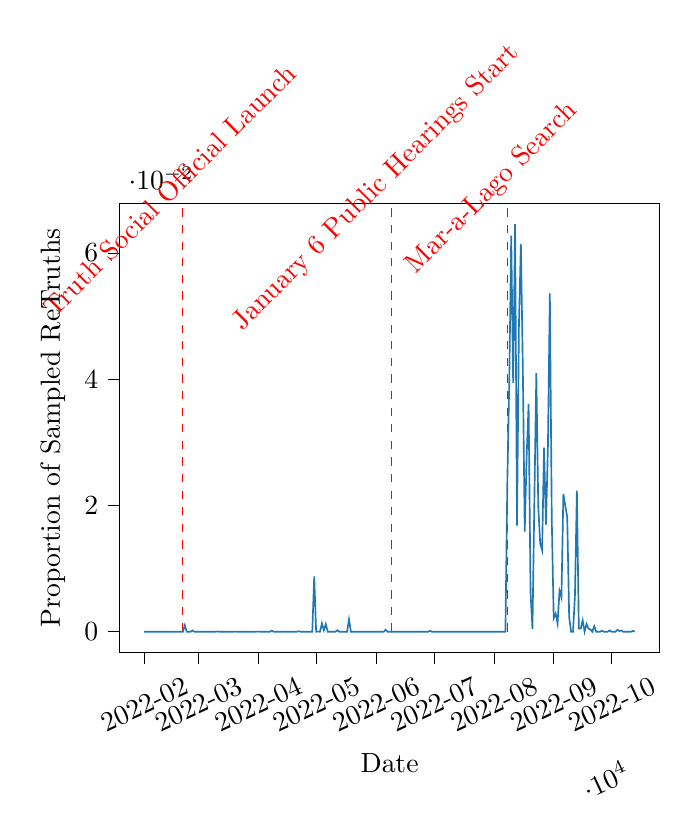
\begin{tikzpicture}

\definecolor{darkgray176}{RGB}{176,176,176}
\definecolor{steelblue31119180}{RGB}{31,119,180}

\begin{axis}[
tick align=outside,
tick pos=left,
x grid style={darkgray176},
xmin=19011.3, xmax=19290.7,
xtick style={color=black},
xtick={19024,19052,19083,19113,19144,19174,19205,19236,19266},
xlabel={Date},
xticklabel style={rotate=25.0},
ylabel={Proportion of Sampled ReTruths},
clip=false,
xticklabels={2022-02,2022-03,2022-04,2022-05,2022-06,2022-07,2022-08,2022-09,2022-10},
y grid style={darkgray176},
ymin=-0.00322825929967097, ymax=0.0677934452930903,
ytick style={color=black}
],
\addplot +[red, dashed, mark=none] coordinates
{(19044, 0) (19044, 0.0677934452930903)} node[above, rotate=45] {Truth Social Official Launch};
\addplot +[red, dashed, mark=none] coordinates
{(19152, 0) (19152, 0.0677934452930903)} node[above, rotate=45] {January 6 Public Hearings Start};
\addplot +[red, dashed, mark=none] coordinates
{(19212, 0) (19212, 0.0677934452930903)} node[above, rotate=45] {Mar-a-Lago Search};

\addplot [semithick, steelblue31119180]
table {%
19024 0
19025 0
19026 0
19027 0
19028 0
19029 0
19030 0
19031 0
19032 0
19033 0
19034 0
19035 0
19036 0
19037 0
19038 0
19039 0
19040 0
19041 0
19042 0
19043 0
19044 0
19045 0.00102921739425944
19046 0
19047 0
19048 0
19049 0.000199046760210553
19050 0
19051 0
19052 3.64109927214426e-06
19053 0
19054 0
19055 0
19056 1.21369975738142e-06
19057 0
19058 0
19059 0
19060 0
19061 0
19062 4.00520919935868e-05
19063 0
19064 0
19065 0
19066 0
19067 0
19068 0
19069 0
19070 0
19071 1.57780968459584e-05
19072 0
19073 0
19074 0
19075 0
19076 0
19077 0
19078 0
19079 0
19080 0
19081 0
19082 7.28219854428851e-06
19083 2.42739951476284e-05
19084 0
19085 0
19086 0
19087 0
19088 0
19089 0
19090 0.00017962756409245
19091 0
19092 0
19093 0
19094 0
19095 0
19096 1.09232978164328e-05
19097 0
19098 0
19099 0
19100 0
19101 0
19102 0
19103 0
19104 7.64630847150294e-05
19105 0
19106 0
19107 0
19108 0
19109 0
19110 0
19111 0
19112 0.00876291224829384
19113 0
19114 1.94191961181027e-05
19115 0
19116 0.00132900123433265
19117 0.000231816653659851
19118 0.00122098195592571
19119 0
19120 0
19121 0
19122 0
19123 0
19124 0.000231816653659851
19125 0
19126 0
19127 0
19128 0
19129 0
19130 0.00194191961181027
19131 0
19132 0
19133 0
19134 0
19135 0
19136 0
19137 0
19138 0
19139 0
19140 0
19141 0
19142 0
19143 0
19144 0
19145 0
19146 0
19147 0
19148 0
19149 0.000324057835220839
19150 0
19151 0
19152 0
19153 0
19154 0
19155 0
19156 0
19157 0
19158 0
19159 0
19160 0
19161 0
19162 0
19163 0
19164 0
19165 0
19166 0
19167 0
19168 0
19169 0
19170 0
19171 0
19172 0.000152926169430059
19173 0
19174 0
19175 0
19176 0
19177 0
19178 0
19179 0
19180 0
19181 0
19182 0
19183 0
19184 0
19185 0
19186 1.21369975738142e-06
19187 0
19188 0
19189 0
19190 0
19191 0
19192 0
19193 0
19194 0
19195 0
19196 0
19197 0
19198 0
19199 0
19200 0
19201 0
19202 0
19203 0
19204 0
19205 0
19206 0
19207 0
19208 0
19209 0
19210 0
19211 0
19212 0.0239657154092535
19213 0.0397802232479334
19214 0.0627628418537079
19215 0.0393979078243582
19216 0.0645651859934193
19217 0.0168133827390048
19218 0.0486402314768177
19219 0.0614544735152507
19220 0.0419163348209247
19221 0.0158666969282473
19222 0.0279223766183169
19223 0.0360857211864643
19224 0.00619108246240262
19225 0.000450282609988506
19226 0.0210504085920233
19227 0.0409465887147769
19228 0.0198524869314879
19229 0.0139842486045487
19230 0.0129089106195088
19231 0.0291785558672067
19232 0.0169711637074644
19233 0.0292076846613838
19234 0.0535787757896027
19235 0.0177163753584966
19236 0.00214339377153558
19237 0.00288132322402349
19238 0.00130351353942764
19239 0.00649450740174797
19240 0.00542038311646542
19241 0.0218332449355343
19242 0.0198961801227536
19243 0.0181581620701834
19244 0.00230360213950993
19245 0
19246 0
19247 0.00577842454489293
19248 0.0223660591290248
19249 0.000496403200769
19250 0.000486693602709949
19251 0.0017962756409245
19252 0
19253 0.00123797375252905
19254 0.000481838803680423
19255 0.000360468827942281
19256 1.21369975738142e-06
19257 0.00088114602385891
19258 6.06849878690709e-06
19259 0
19260 1.21369975738142e-06
19261 0.00014564397088577
19262 1.21369975738142e-06
19263 0
19264 0
19265 0.00021361115729913
19266 0
19267 0
19268 0
19269 0.000311920837647025
19270 0.000110446677921709
19271 0.000201474159725315
19272 0
19273 0
19274 0
19275 0
19276 1.21369975738142e-06
19277 0.000143216571371007
19278 0
};
\end{axis}

\end{tikzpicture}
